% Four faults, six tools, and the column of silence down the left.
%
% This is the argument for the whole project in one drawing. Only the
% first fault announces itself. The other three produce no symptom at the
% moment they happen, so the tool has to be in place and understood
% beforehand, because afterwards there is nothing to look at.
\documentclass[tikz, border=4pt]{standalone}
% Shared styles for the Project 9 figures.
%
% Every figure in this directory is standalone: it inputs this file and
% compiles on its own with
%
%     pdflatex arch.tex
%
% so a reader can render one drawing without building a book around it.
%
% The palette carries the distinction this project keeps confusing when it
% is drawn in one colour: what runs on the target, what runs on the host,
% and which of the two halves of the serial cable a given box is talking
% to. The fourth colour is for a fault that produces no symptom, which is
% three of the four faults here and the reason the project exists.
\usepackage{tikz}
\usepackage[siunitx]{circuitikz}
\usetikzlibrary{arrows.meta, backgrounds, calc, fit, positioning, shapes.geometric, shapes.misc}

\definecolor{usercol}{RGB}{222, 235, 247}   % target, user space
\definecolor{kerncol}{RGB}{198, 219, 239}   % target, kernel
\definecolor{hostcol}{RGB}{229, 245, 224}   % host, off the board
\definecolor{toolcol}{RGB}{254, 217, 118}   % a debugging tool
\definecolor{hwcol}{RGB}{229, 229, 229}     % hardware, files, RAM
\definecolor{quietcol}{RGB}{245, 245, 245}  % a fault with no symptom
\definecolor{linecol}{RGB}{70, 70, 70}
\definecolor{badcol}{RGB}{200, 60, 60}
\definecolor{okcol}{RGB}{60, 140, 70}

\tikzset{
  blk/.style   = {draw=linecol, rounded corners=2pt, align=center,
                  font=\sffamily\small, inner sep=4pt, minimum height=9mm},
  user/.style  = {blk, fill=usercol},
  kern/.style  = {blk, fill=kerncol},
  host/.style  = {blk, fill=hostcol},
  tool/.style  = {blk, fill=toolcol},
  hw/.style    = {blk, fill=hwcol},
  quiet/.style = {blk, fill=quietcol, draw=linecol!50, dashed},
  bad/.style   = {blk, fill=white, draw=badcol, thick, text=badcol},
  layer/.style = {draw=linecol!40, dashed, rounded corners=3pt, inner sep=6pt},
  layerlabel/.style = {font=\sffamily\scriptsize\bfseries, inner sep=2pt},
  lbl/.style   = {font=\sffamily\scriptsize, fill=white, inner sep=1pt},
  flow/.style  = {-{Stealth[length=2mm]}, draw=linecol, thick},
  bus/.style   = {{Stealth[length=2mm]}-{Stealth[length=2mm]}, draw=linecol,
                  thick},
  % The serial line is drawn thick and dark everywhere it appears, because
  % the single point of this project's host side is that it is one wire.
  wire/.style  = {{Stealth[length=2mm]}-{Stealth[length=2mm]}, draw=linecol,
                  very thick},
  % UML sequence
  actor/.style = {blk, fill=usercol, font=\sffamily\scriptsize,
                  minimum height=6mm},
  lifeline/.style = {draw=linecol!50, dashed},
  msg/.style   = {-{Stealth[length=1.6mm]}, draw=linecol},
  reply/.style = {-{Stealth[length=1.6mm]}, draw=linecol, dashed},
  umlnote/.style = {draw=linecol!60, fill=yellow!12, rounded corners=1pt,
                    font=\sffamily\scriptsize, align=left, inner sep=3pt},
  activation/.style = {draw=linecol, fill=usercol, minimum width=2mm},
  % decision tree
  qst/.style   = {draw=linecol, fill=white, diamond, aspect=2.6, align=center,
                  font=\sffamily\scriptsize, inner sep=1pt},
  ans/.style   = {font=\sffamily\scriptsize\itshape, inner sep=1pt},
  fix/.style   = {blk, fill=hostcol, font=\sffamily\scriptsize, align=left},
  trans/.style = {-{Stealth[length=1.6mm]}, draw=linecol},
  % fault matrix
  cell/.style  = {draw=linecol!40, minimum width=17mm, minimum height=7mm,
                  font=\sffamily\scriptsize, align=center},
  hit/.style   = {cell, fill=okcol!25},
  miss/.style  = {cell, fill=badcol!12, text=badcol},
  head/.style  = {cell, font=\sffamily\scriptsize\bfseries, fill=hwcol},
}


\begin{document}
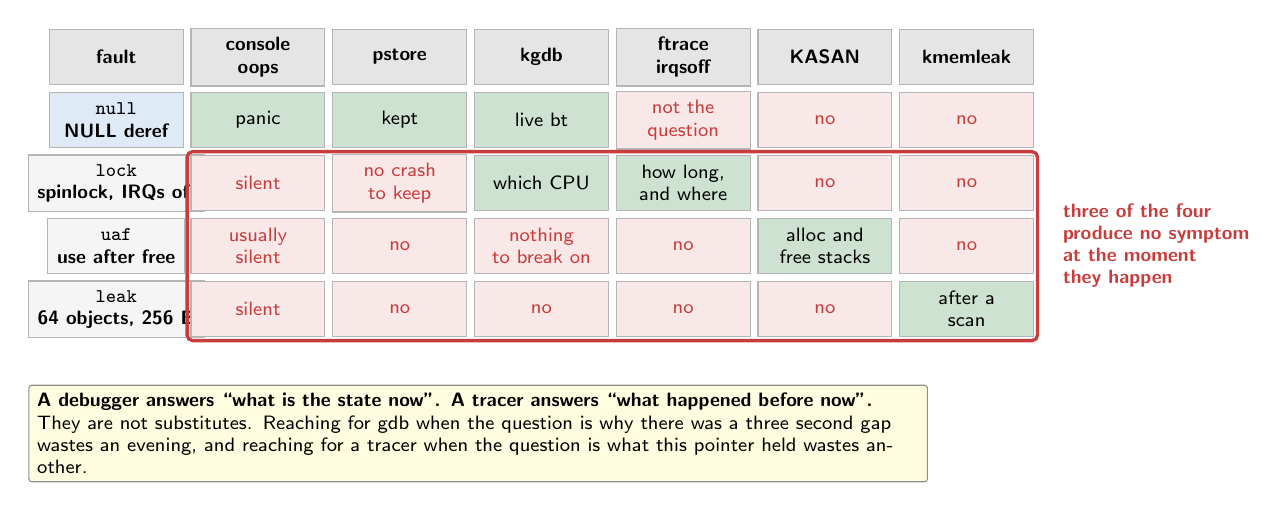
\begin{tikzpicture}[x=18mm, y=8mm]

  %% ---------------- column headings ----------------
  \node[head] at (0,0) {fault};
  \node[head] at (1,0) {console\\oops};
  \node[head] at (2,0) {pstore};
  \node[head] at (3,0) {kgdb};
  \node[head] at (4,0) {ftrace\\irqsoff};
  \node[head] at (5,0) {KASAN};
  \node[head] at (6,0) {kmemleak};

  %% ---------------- row 1: null ----------------
  \node[head, fill=usercol] at (0,-1)
       {\texttt{null}\\\scriptsize NULL deref};
  \node[hit]  at (1,-1) {panic};
  \node[hit]  at (2,-1) {kept};
  \node[hit]  at (3,-1) {live bt};
  \node[miss] at (4,-1) {not the\\question};
  \node[miss] at (5,-1) {no};
  \node[miss] at (6,-1) {no};

  %% ---------------- row 2: lock ----------------
  \node[head, fill=quietcol] at (0,-2)
       {\texttt{lock}\\\scriptsize spinlock, IRQs off};
  \node[miss] at (1,-2) {silent};
  \node[miss] at (2,-2) {no crash\\to keep};
  \node[hit]  at (3,-2) {which CPU};
  \node[hit]  at (4,-2) {how long,\\and where};
  \node[miss] at (5,-2) {no};
  \node[miss] at (6,-2) {no};

  %% ---------------- row 3: uaf ----------------
  \node[head, fill=quietcol] at (0,-3)
       {\texttt{uaf}\\\scriptsize use after free};
  \node[miss] at (1,-3) {usually\\silent};
  \node[miss] at (2,-3) {no};
  \node[miss] at (3,-3) {nothing\\to break on};
  \node[miss] at (4,-3) {no};
  \node[hit]  at (5,-3) {alloc and\\free stacks};
  \node[miss] at (6,-3) {no};

  %% ---------------- row 4: leak ----------------
  \node[head, fill=quietcol] at (0,-4)
       {\texttt{leak}\\\scriptsize 64 objects, 256 B};
  \node[miss] at (1,-4) {silent};
  \node[miss] at (2,-4) {no};
  \node[miss] at (3,-4) {no};
  \node[miss] at (4,-4) {no};
  \node[miss] at (5,-4) {no};
  \node[hit]  at (6,-4) {after a\\scan};

  %% ---------------- the reading of it ----------------
  \draw[badcol, very thick, rounded corners=2pt]
       (0.5,-1.5) rectangle (6.5,-4.5);
  \node[anchor=west, font=\sffamily\scriptsize\bfseries, text=badcol]
       at ($(6.5,-3)+(2mm,0)$)
       {\begin{tabular}{@{}l@{}}
          three of the four\\
          produce no symptom\\
          at the moment\\
          they happen
        \end{tabular}};

  \node[umlnote, anchor=north west, text width=112mm, align=left]
       at (-0.62,-5.2)
       {\textbf{A debugger answers ``what is the state now''. A tracer
        answers ``what happened before now''.} They are not substitutes.
        Reaching for gdb when the question is why there was a three second
        gap wastes an evening, and reaching for a tracer when the question
        is what this pointer held wastes another.};

\end{tikzpicture}
\end{document}
